\documentclass[10pt]{article}

\usepackage[margin=1in, letterpaper]{geometry}
\usepackage{parskip}

\usepackage{amsthm, amsmath, amssymb}
\usepackage{gensymb}  % For use of degree symbol
\usepackage[pdftex]{graphicx}
\usepackage{hyperref}

\usepackage{enumerate} % For use of (a), (b), et cetera
\usepackage{booktabs} % Tables
\usepackage[margin=20pt, labelfont=bf, labelsep=period,
justification=justified]{caption} % Captions in figure floats

% ======================
% Document setup, layout
% ======================

% The following metadata will show up in the PDF properties
\hypersetup{
	colorlinks = true,
	urlcolor = magenta,  % Links to URLs
	linkcolor = blue,  % Links within PDF
	pdfauthor = {Aaron Tran},
	pdfkeywords = {berkeley},
	pdftitle = {Astro 121, UG Radio Lab, Lab 3 - \today},
	pdfsubject = {},
	pdfpagemode = UseNone
}

% Don't indent paragraphs
\setlength\parindent{0em}

% Slightly more compact lines
\linespread{0.95}

% ===============
% Useful commands
% ===============
\newcommand {\mt}{\mathrm}
\newcommand {\unit}[1]{\; \mt{#1}}
% http://vemod.net/typesetting-units-in-latex

% Sets, operators
\newcommand {\ints}{\mathbb{Z}}
\newcommand {\ptl}{\partial}
\newcommand {\dl}{\nabla}

\begin{document}

% =======
% Titling
% =======
\begin{center}
\Large{Two-element interferometer fringe measurements at $10.7 \unit{GHz}$}

\normalsize
\textbf{Aaron Tran}${}^{1,2,3}$ \\
Leonardo S. Cassara${}^{1,2}$, Ryan (Xin Xing) Gao${}^{1,2}$, Patrick Kantorski${}^{1,2}$, Salman Kahn${}^{1,4}$ \\
Aaron Parsons${}^{2,5,6}$, Garrett K. Keating${}^{2,5,6}$, Baylee Bordwell${}^{2,6}$ \\
\footnotesize
${}^1$PLSAR Collaboration \\
${}^2$Dept. Astronomy, UC Berkeley, D-23 Hearst Field Annex, Berkeley, CA 94720, USA \\
${}^3$Dept. Earth and Planetary Science, UC Berkeley, 335 McCone Hall, Berkeley, CA 94720, USA \\
${}^4$Dept. Physics, UC Berkeley, 251 LeConte Hall, Berkeley, CA 94720, USA \\
${}^5$Radio Astronomy Laboratory, UC Berkeley, Berkeley, CA 94720, USA \\
${}^6$Undergraduate Radio Laboratory teaching staff \\
\textit{Not received 2014 April 7; submitted 2014 April 20; damnatio memoriae 2014 April 20}
\end{center}

% ========
% Abstract
% ========
\section*{Abstract}

We estimate source declinations and angular diameters from $10.7 \unit{GHz}$ interferometer fringe frequencies and modulation.  Declinations fitted from strong radio source fringes (Orion, M17) are accurate to $\sim1\degree$.  We estimate Sun, Moon angular diameters of $\sim0.3$--$0.6\degree$ by matching zero crossings in expected modulation functions with fringe envelope minima.  Envelope fits are limited by noise and poor low-altitude signal and are hence less robust than fringe frequency fits.

\textit{Keywords}: astrometry --- instrumentation: interferometers --- galaxies: individual (NGC 4486) --- ISM: individual (NGC 1976, NGC 6618)

% ============
% Introduction
% ============
\section{Introduction}

Radio interferometers can achieve large beamwidth and fine angular resolution by careful array design, enabling study of molecular transitions in star forming regions, various sources of radio continuum emission, the $21 \unit{cm}$ line, and much more.  The budding radio astronomer had better start with a nice two element array, if he or she is to ever have hope of understanding larger arrays.  Here we present point and extended source observations from a 2 element interferometer with baseline $B=10\unit{m}$ operating at $10.7\unit{GHz}$.  The compete procedure of data acquisition, processing, and model fitting provides a template for understanding 1-D interferometer observation.  The same principles operate for more sophisticated 2-D arrays and even very long baseline interferometry.

We introduce astronomical coordinates (space and time) at an elementary level, so that we may calculate object ephemerides and perform telescope tracking.  Data reduction recovers the interferometer fringes and fringe modulation.  We perform non-linear least squares fitting to determine fringe frequencies and minima in fringe modulation.  From these procedures we may estimate source declinations, interferometer baseline, and/or source angular extents.  Fringe amplitudes may also enable estimation of source strength, but for all sources but Sun and Moon the fringe sinusoid is covered by noise.

% =================
% Rotation matrices
% =================
\section{Review of astronomical time and coordinates}

We review astronomical timekeeping and coordinate systems used in this study: sidereal time, Julian dates, right ascension and declination, and altitude-azimuth coordinates.
A far more thorough and pedagogical presentation is given by \textit{Green} [1985].
For sanity's sake, I assume the reader is acquainted with geographical and celestial coordinates.

\emph{Julian date} quantifies solar time; a Julian day is $86400 \unit{seconds}$ and a Julian year is $365.25 \unit{days}$.
The timescales used to measure Julian dates may vary (e.g. ephemeris time, terrestrial dynamical time) and are difficult to decipher.
\emph{Sidereal time} quantifies Earth's rotation relative to the fixed stars.
As viewed from Earth, the fixed stars take one \emph{sidereal day} (23h, 56m, 4s of solar time) to sweep out $360\degree$ longitude on the celestial sphere.
A sidereal day is slightly shorter than a solar day due to the Earth's orbital motion around the Sun, and, to a much lesser extent, precession and nutation of the Earth's rotation axis.
\emph{Local sidereal time} (LST) is sidereal time adapted for a specific location (longitude) on Earth, and is defined by the vernal equinox's hour angle (HA).

Astronomical positions are specified by location-agnostic spherical coordinates, typically \emph{right ascension} (RA, $\alpha$) and \emph{declination} (dec, $\delta)$.
To perform observations, we convert $(\alpha, \delta)$ into more useful coordinates for given geographic latitude and longitude -- namely, \emph{altitude} and \emph{azimuth} (alt, az).  \emph{Hour angle} $h_s$ will also be useful.
Our presentation of the requisite coordinate transformation follows that of Carl Heiles.

Let $(x,y,z)$ specify a right-handed coordinate system where the polar angle is measured relative to the $z$-axis and the azimuth is measured in the $x$-$y$ plane starting from the positive $x$-axis.
In $(\alpha, \delta)$ coordinates, the Earth's rotation axis and equatorial plane correspond to the $z$-axis and $x$-$y$ plane respectively (i.e., right ascension and declination specify a geocentric equatorial coordinate system).
Right ascension is measured counter-clockwise about the $z$-axis starting from the vernal equinox's position on the celestial sphere (positive $x$-axis).
Declination is measured upwards (towards positive $z$) from the equatorial ($x$-$y$) plane.
We see that declination corresponds to the usual polar angle, and right ascension to azimuthal angle.

We compute coordinate transformations using rotation matrices in Cartesian coordinates.
Our coordinate transformations act upon Cartesian coordinate bases from which we measure polar and azimuthal angles for (RA, dec), (HA, dec), and (alt, az) coordinates (e.g., our previously defined $x,y,z$); these transformations are deemed ``passive'' as they only alter the coordinate representations of physical vectors.
A unit vector in $(\alpha, \delta)$ coordinates may be written in Cartesian coordinates as:
\[
	(x, y, z) = (\cos\alpha\cos\delta, \sin\alpha\cos\delta, \sin\delta)
\]
We select a longitude by converting right ascension ($\alpha$) to hour angle ($h_s$):
\[
	h_s = \mathrm{LST} - \alpha
\]
This transformation is a rotation about the $z$-axis and a reflection across the $x$-$z$ plane; (HA, $\delta$) coordinates have reversed handedness compared to $(\alpha, \delta)$ and the rotated $x$-axis is perpendicular to the meridian at which we evaluate LST, HA.
The new coordinate basis has Cartesian representation:
\[
	(x', y', z') = (\cos(h_s)\cos\delta, \sin(h_s)\cos\delta, \sin\delta)
\]
Two more rotations convert (HA, $\delta$) to (alt, az).
We rotate the $x'$-$z'$ plane by $(\phi - \pi /2)$, where $\phi$ is geographic latitude, then rotate the transformed $x'$-$y'$ plane by $\pi$ radians.
The rotation matrix is constructed as:
\[
	\begin{pmatrix}
		\cos(\pi) & \sin(\pi) & 0 \\
		\sin(\pi) & \cos(\pi) & 0 \\
		0 & 0 & 1
	\end{pmatrix}
	\begin{pmatrix}
		\cos\left(\phi-\pi/2\right) & 0 & \sin\left(\phi-\pi/2\right) \\
		0 & 1 & 0 \\
		\sin\left(\phi-\pi/2\right) & 0 & \cos\left(\phi-\pi/2\right)
	\end{pmatrix}
	=
	\begin{pmatrix}
		-\sin\phi & 0 & \cos\phi \\
		0 & -1 & 0 \\
		\cos\phi & 0 & \sin\phi
	\end{pmatrix}
\]
The final coordinate basis has the same handedness as (HA, $\delta$) coordinates and is written:
\[
	(x'', y'', z'') = (\cos(\mathrm{az})\cos(\mathrm{alt}),
					   \sin(\mathrm{az})\cos(\mathrm{alt}),
					   \sin(\mathrm{alt}))
\]
Altitude is measured upwards from the $x''$-$y''$ plane (i.e., the Earth's local tangent plane) and azimuth is measured clockwise from geographic north.

For arbitrary $(\alpha, \delta)$, the topocentric Cartesian coordinates are:
\[
	\hat{s} =
	\begin{pmatrix}
		-\cos(h_s) \sin\phi \cos\delta + \cos\phi \sin\delta \\
		-\sin(h_s) \cos\delta \\
		 \cos(h_s) \cos\phi \cos\delta + \sin\phi \sin\delta
	\end{pmatrix}
\]

These coordinate transformations correctly predict astronomical positions for both stationary celestial objects and Solar System objects.
Our rotation matrices agree with PyEphem calculations to $\sim 10 \unit{arcseconds}$; note that PyEphem's atmospheric refraction correction must be disabled.
In this study, we use PyEphem to compute all coordinate transformations for observations and data analysis.


% =======
% Methods
% =======
\section{Methods}

% ---------------------
% Interferometer design
% ---------------------
\subsection{Interferometer design}

We measure $10.7 \unit{GHz}$ (X-band) emission using a two-element multiplying interferometer.
The interferometer consists of two antennae (diameter $d \sim 1 \unit{m}$) with east-west baseline $B \approx 10 \unit{m}$ on the rooftop of Wurster Hall, Univ. California Berkeley ($37\degree 52' 12.7'' \unit{N}$, $-122\degree 15' 15.8'' \unit{E}$).
The interferometer beam size is $\lambda/d \sim 1.6\degree$ and angular resolution is $\lambda / B \sim 0.16\degree$.
The stated bandwidth is $10 \unit{MHz}$, though we do not know the antenna response or the frequency band uncertainty of our interferometer dishes.
We conservatively estimate the absolute frequency error to be $\sim 100 \unit{MHz}$ at worst.

The interferometer may point from $15\degree$ to $87\degree$ in altitude, and its northern field of view is obstructed by a taller portion of Wurster Hall.
We estimate that Wurster Hall obstructs the sky between $-20\degree$ and $10\degree$ azimuth and up to $40\degree$ altitude.
All observations are performed within $17$--$85\degree$ altitude and outside the range of the Wurster Hall obstruction.

A fixed celestial object will move at most $15\degree$ per hour, or $0.125\degree$ every $30 \unit{s}$.
We point the interferometer at $30 \unit{second}$ intervals to keep point sources of interest within $\sim 0.13\degree$ ($10\%$ of interferometer beamwidth) of the interferometer beam's center.
Encoders in the interferometer dishes must be reset (``homed'') every 100 pointings to maintain angular positioning accuracy.
Homing takes $\sim 1 \unit{minute}$ for every $50 \unit{min.}$ of observation.
Interferometer data collected while homing appear as voltage spikes which we  remove during data reduction.

% -----------------
% Signal processing
% -----------------
\subsection{Interferometer signal processing}

The interferometer signal is heterodyne downconverted at the dishes to approximately $1.7 \unit{GHz}$, then to $150 \unit{MHz}$ further along the signal path.
The twice-downconverted signals are mixed and sampled at $\sim 1 \unit{Hz}$.
Amplifiers and filters between downconverting mixers improve signal quality and restrict signal bandwidth to $10 \unit{MHz}$.
But, we necessarily lose information about electric field amplitude at the interferometer dishes.

% ============
% Observations
% ============
\section{Observations}

% Observing campaign
\subsection{Observing campaign}

We observed the Sun, the Moon, and the unresolved point sources NGC 1976 (Orion Nebula, M42), NGC 4486 (Virgo A, M87), and NGC 6618 (Omega Nebula, M17) (Table~\ref{tab:obs}).  The Moon was observed twice: once while waxing crescent with $\sim20\%$ illumination (2014 April 4), and once during a total lunar eclipse (2014 April 15).
All observations are single horizon-to-horizon runs except our observation of the Orion Nebula.

\begin{table}[!ht]
\centering
\caption{Summary of interferometer observations.  Sun and moon flux densities are calculated with $T_b = 14600 \unit{K}$, $217 \unit{K}$ assuming uniform blackbody emission.  Sun brightness temperature is average of estimates for sunspot cycle minima and maxima [\textit{Hafez et al.}, 2014; \textit{Salomonovich and Losovskii}, 1963].}
\label{tab:obs}
\begin{tabular}{@{}rrrr@{}}
    \toprule
    Object & $S_\nu$ (Jy) & Observation start (UT) & Observation end (UT) \\
    \midrule
    Sun & $\sim 4 \cdot 10^6$ & 2014 Apr 01 15:25:44 & 2014 Apr 02 01:02:20 \\
    Moon & $\sim 6 \cdot 10^4$ & 2014 Apr 04 18:54:38 & 2014 Apr 05 06:09:51 \\
    (eclipsed) Moon & $\sim 6 \cdot 10^4$ & 2014 Apr 15 04:09:22 & 2014 Apr 15 12:06:06 \\
    NGC 1976 & $\sim 340$ & 2014 Mar 21 22:53:18 & 2014 Mar 22 09:01:47 \\
    NGC 4486 & $\sim 34$ & 2014 Apr 03 03:03:15 & 2014 Apr 03 12:57:36 \\  % From cut at last pointing
    NGC 6618 & $\sim 500$ & 2014 Apr 05 10:07:34 & 2014 Apr 05 17:04:13 \\
    \bottomrule
\end{tabular}
\end{table}

% --------------
% Data reduction
% --------------
\subsection{Data reduction}

Dish homing takes $\sim1 \unit{minute}$ and introduces spurious voltage spikes as data collection continues during homing and subsequent re-pointing.  We extract homing start and stop times from automatically generated observing logs and remove all data associated with homing and re-pointing (Figure~\ref{fig:reduction}a).  The interferometer output also carries a fluctuating DC offset ($\Delta V \sim \pm 1 \unit{mV}$) comparable to measured voltages for all sources except the sun; we are unable to explain the cause of this variable offset.  We extract the DC offset signal with a $240 \unit{second}$ wide boxcar filter and subtract the offset from the interferometer output.  Figure~\ref{fig:reduction} plots raw and reduced data for the 2014 April 4 moon observation.

\begin{figure}[!ht]
    \centering
    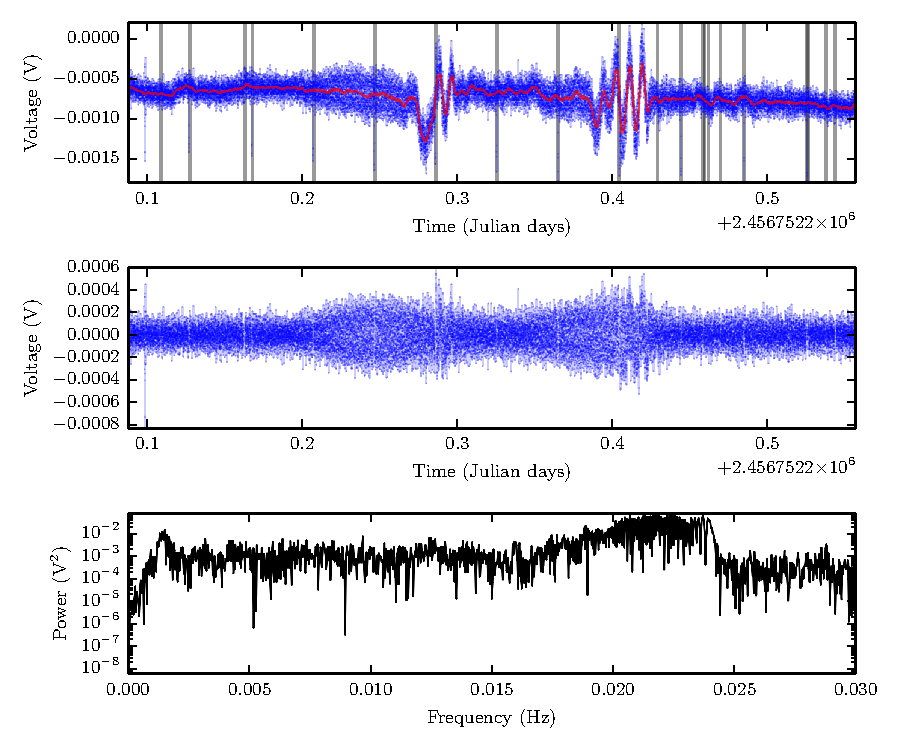
\includegraphics{plots/moon_cleaning.pdf} \\
    \caption{(top) Raw interferometer output from 2014 April 4 Moon observation; overlaid vertical lines identify homing spikes and gaps in data collection.  Red curve plots boxcar-smoothed signal to be subtracted. (middle) Interferometer output with fluctuating offset and homing spikes removed.  Data reduction allows fringe modulation to be recovered and extracted.  (bottom) Partial power spectrum of reduced interferometer data.}
    \label{fig:reduction}
\end{figure}

We compute power spectra as a function of frequency from cleaned data using the discrete Fourier transform.  For moon and sun observations, we observe a gradually increasing signal from $0.015$--$0.027 \unit{Hz}$ consistent with the range of expected fringe frequencies; in point source data, a weak and possibly spurious peak may be discerned near $0.027 \unit{Hz}$.  We assume the sampling period is $1 \unit{second}$ despite gaps in data sampling, introducing some error.  Although we do not account for uneven sampling here, the interested reader may refer to work by \textit{Dutt and Rokhlin} [1993] and \textit{Ferraz-Mello} [1981].

% =======
% Results
% =======
\section{Results}

% ---------------------
% Interferometer signal
% ---------------------
\subsection{Interferometer point source response}

The interferometer outputs the product of two voltage signals.  For a point source, the interferometer response is proportional to:
\begin{align*}
	F(t) &= \cos(2\pi\nu t) \cos\left(2\pi\nu \left[ t + \tau \right] \right) \\
		 &\approx \cos\left(2\pi\nu \tau\right)
\end{align*}
where the time delay $\tau = (B_y / c) \cos\delta \sin(h_s) + \tau_c$ sums geometric and cable delay and we have dropped a rapidly varying $22 \unit{GHz}$ sum term.
Splitting $\tau$ into cable and geometric delays gives:
\begin{equation} \label{eq:ptfringe}
	F(t) = \cos(2\pi\nu\tau_c)
			\cos \left[2\pi \left(\frac{B_y}{\lambda}\cos\delta\right)
			           \sin h_s \right]
			- \sin(2\pi\nu\tau_c)
			\sin \left[2\pi \left(\frac{B_y}{\lambda}\cos\delta\right)
			           \sin h_s \right]
\end{equation}
As $\tau_c$ is a constant, the interferometer output is a sinusoid with time-dependent frequency determined by $\sin(h_s)$.  This is the \emph{fringe frequency} $f_f$, which we calculate by Taylor expanding the sin/cos argument in hour angle:
\[
    2\pi \frac{B_y}{\lambda}\cos\delta \sin (h_s + \Delta h)
    = 2\pi \frac{B_y}{\lambda}\cos\delta \left[
        \sin (h_s) + \cos (h_s) \Delta h + O\left((\Delta h)^2\right)
      \right]
\]
The $\Delta h$ term captures time dependence, while the first term is simply a phase argument.  The local fringe frequency is then:
\[
    f_f = 2\pi \frac{B_y}{\lambda} \cos\delta \cos\left(h_s\right)
\]

% ----------------------
% Dec / baseline fitting
% ----------------------
\subsection{Declination measurement from fringe frequencies}

We may infer either of interferometer baseline or source declination by non-linear least squares fitting our interferometer data to equation~\ref{eq:ptfringe}.  Our non-linear fit involves three free parameters: $A \equiv \cos(2\pi\nu\tau_c)$, $B \equiv \sin(2\pi\nu\tau_c)$, and $k \equiv 2\pi \frac{B_y}{\lambda}\cos\delta$.  We compute $x \equiv \sin h_s$ from the times and hence hour angles of all observations.  The fit equation becomes:
\[
    F(t) = A \cos(k x) + B \sin(k x)
\]
If a value of $k$ is given, $A$ and $B$ are readily fit by linear least squares.  We brute force the non-linear least squares fit in $k$ as follows.

\begin{figure}[!ht]
    \centering
    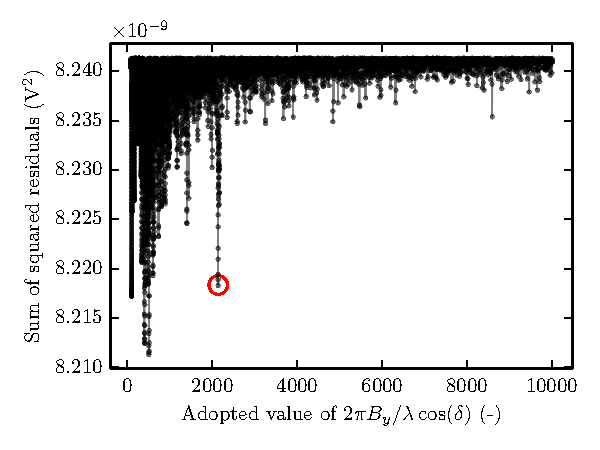
\includegraphics{plots_fitting/M17_dec_fits_lsq_logk.pdf}
    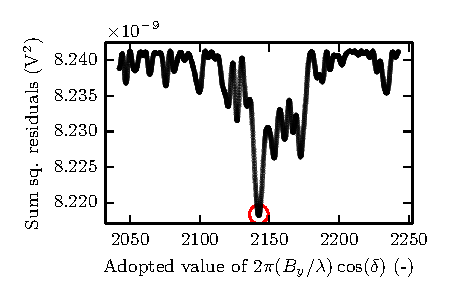
\includegraphics{plots_fitting/M17_dec_fits_lsq.pdf}
    \caption{Scaled sum of squared residuals from linear fits for $A,B$ as a function of $k = 2\pi \left(B_y/\lambda\right) \cos\delta$, fitting fringe data from NGC 6618 (M17); (left) a large range of possible $k$ values with logarithmic sampling; (right) a smaller range of $k$ values shows nearby minima.  Red circles plot iteratively computed best-fit $k$.  Note that ordinate ($y$) axes differ between the two plots.}
    \label{fig:declsq}
\end{figure}

% Goddammit this is horribly explained
We seek a value of $k$ that minimizes the sum of squared residuals, computed from a linear fit to $A,B$.  Start with an initial guess $k_i = 2000$ and search domain $k\in[1000, 3000]$ centered on $k_i$.  Sample $1000$ evenly spaced $k$ values in this range and use each value to compute a linear least squares fit for $A,B$.  Take the sampled $k$ value with minimum sum of squared residuals as our next guess for $k$ and halve the search domain.  Iterate this procedure of guessing $k$ and refining the search domain until two consecutive guesses for $k$ differ by less than $0.0002$ (i.e., fractional change $\sim 10^{-7}$ for $k \approx 2000$).  Our procedure converges to a value of $k$ within or near the initial search domain (Figure~\ref{fig:declsq}), although it is not guaranteed to converge to an absolute minimum within or near the search domain.  Qualitatively, our procedure appears robust to variations in sampling and search domain.

\begin{figure}[!ht]
    \centering
    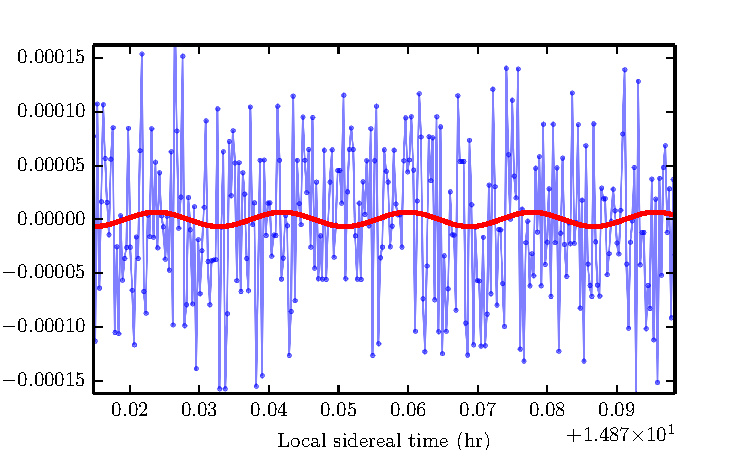
\includegraphics{plots_fitting/M17_dec_fits_signal.pdf}
    \caption{Red line plots equation~\ref{eq:ptfringe} with best fit values for $k,A,B$ from non-linear least squares fitting procedure; blue circles plot interferometer data from NGC6618 (M17), corresponding to fit $k$ from Figure~\ref{fig:declsq}.}
    \label{fig:decsig}
\end{figure}

Our fits are only marginally better than a straight line fit and cannot explain most sample variance (Figure~\ref{fig:decsig}).  However, Figure~\ref{fig:declsq} illustrates that a meaningful signal is present and can be robustly detected by our non-linear fitting procedure.  With a value for $k$ in hand, we assume baseline $B = 10 \unit{m}$ and estimate the fit declination $\delta$.  We also perform the reverse procedure by calculating source declinations (epoch J2000, precessed to 2014 April 7 using PyEphem) and then estimate the fit baseline.  We estimate the cable delay by computing $2\pi\nu\tau_c = \arctan(-B/A)$ (equation~\ref{eq:ptfringe}); however, the largest measurable cable delay is $\pm 47 \unit{ps}$ as we can only measure signal phase offset.  Table~\ref{tab:dec} summarizes our best fit parameters.

We estimate uncertainties in our fit values by taking $\nu = 10.7 \pm 0.1 \unit{GHz}$ and $B = 10 \pm 0.1 \unit{m}$.  We are unable to quantify uncertainty for our fitted value of $k$, although this is the most important possible source of systematic error.  Interestingly, we expect a more precise measurement of $\delta$ with larger declination (farther from $\delta=0$).  Why?  The function $\cos\delta$ is relatively insensitive to changes in $\delta$ near $\delta=0$, hence uncertainty in $\cos\delta$ is propagated into a larger uncertainty in $\delta$.

\begin{table}[!ht]
\centering
\caption{Parameter estimates from brute force least squares.}
\label{tab:dec}
\begin{tabular}{@{}rrrrr@{}}
    \toprule
    Object & Fit $k$ (-)
        & Fit, actual $\delta$ ($\degree$)
        & Fit $B$ (m) & Fit $\tau_c$ (ps) \\
    \midrule
    NGC 1976 (Orion) & $2227.45$
        & $-6.7\degree \pm 7\degree$, $-5.34\degree$
        & $9.98 \pm 0.1$ & $-27$ \\
    NGC 4486 (Virgo A) & $2077.17$
        & $22.1\degree \pm 2\degree$, $12.31\degree$
        & $9.48 \pm 0.1$ & $42$ \\
    NGC 6618 (M17) & $2142.41$
        & $-17.2\degree \pm 3\degree$, $-16.2\degree$
        & $9.95 \pm 0.1$ & $34$ \\
    \bottomrule
\end{tabular}
\end{table}

The calculated declinations for NGC 1976 (Orion) and NGC 6618 (M17) are accurate to about $1\degree$ on the sky, whereas our estimate of declination for NGC 4486 is off by $10\degree$.  Similarly, the calculated baselines for Orion and M17 agree with expectation to within $0.1 \unit{m}$.  We attribute the poor parameter fits for Virgo A to comparatively weak signal strength; the flux density of Virgo A at $10.7 \unit{GHz}$ is an order of magnitude weaker than flux densities for Orion and M17.  The various estimates of cable delay disagree, as expected.  As the cable delay fit is determined by hour angle phase in equation~\ref{eq:ptfringe}, inconsistent right ascensions may cause our cable delay estimates to differ.  However, we suggest that uncertainty in our fitting procedure greatly outweighs error from inaccurate right ascensions -- i.e., cable delay estimates are not physically meaningful unless we can quantify the robustness (uncertainty) of our non-linear fits.

% ----------------------
% Extended source theory
% ----------------------
\subsection{Interferometer extended source response}

The interferometer response to extended sources in the sky is proportional to:
\[
    R(h_s) = \int I_\nu (\Delta h) \cos(2\pi\nu \tau) d(\Delta h)
\]
Here $h_s$ is the hour angle of the extended source's center, and $\Delta h = h - h_s$ is hour angle $h$ measured relative to our source.  The impulse response is integrated over source extent within antenna beamwidth; for $I_\nu(h_s) = \delta(\Delta h)$, we recover the point source response $F(h_s) = \cos(2\pi\nu \tau)$.  Or, we may think of this as a cosine Fourier transform of source intensity -- a 1-D visibility equation.  To obtain a 1-D intensity distribution $I_\nu$, we simply integrate source specific intensity perpendicular to the baseline direction.  For a symmetric source of small angular extent, Taylor expansion in hour angle gives:
\[
    R(h_s) \approx \cos(2\pi\nu \tau_{\mathrm{tot}}(h_s)) \int I_\nu (\Delta h) \cos(2\pi f_f \Delta h) d(\Delta h)
\]
The left-hand $\cos$ term is simply the point source fringe response; the right-hand integral is a modulation function.  This modulation function should predict our interferometer output's envelope curve (Figure~\ref{fig:sunFringes}).

The modulation function depends on the angular diameter of the source.  Consider a circular source of angular radius $R$ and uniform specific intensity; its 1-D intensity distribution is $I_\nu(\Delta h) = \frac{1}{R} \left( R^2 - (\Delta h)^2 \right)^{1/2}$.  The corresponding modulation function is:
\begin{align*}
    \mathrm{MF} &= \int \frac{1}{R} \left( R^2 - (\Delta h)^2 \right)^{1/2} \cos(2\pi f_f \Delta h) d(\Delta h) \\
                &\propto \frac{1}{2\pi f_f R} \left(2\pi f_f R\right)
                         \int_0^\pi \sin^2 \theta \cos\left(2\pi f_f R \cos(\theta)\right) d\theta \\
                &\propto \frac{1}{2\pi f_f R} J_1 \left(2\pi f_f R \right)
\end{align*}
where $J_1(z)$ is a Bessel function of the first kind [\textit{Abramowitz and Stegun}, 1964].

% ----------------
% Diameter fitting
% ----------------
\subsection{Angular diameters of the Sun, Moon}

\begin{figure}[!ht]
    \centering
    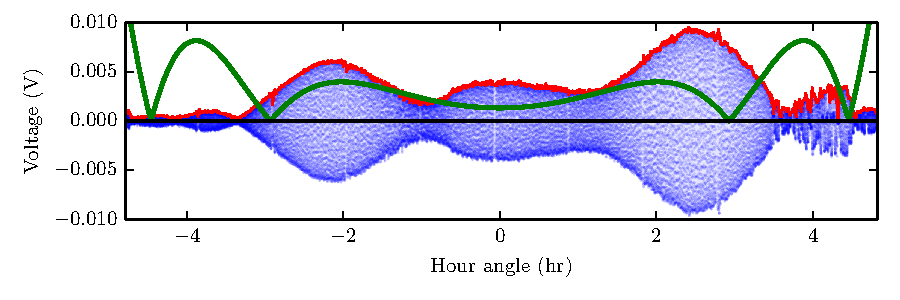
\includegraphics[scale=1]{plots_fitting/sun_fringes_envelopes.pdf} \\
    \caption{Sun observation data with extracted envelope curve (red) and expected modulation function shape (green).}
	\label{fig:sunFringes}
\end{figure}

We estimate source angular diameters from modulation functions of 1 observation of the Sun and 2 observations of the Moon.  Although the theoretical modulation function should describe our fringe envelopes throughout observation, spurious signals from noise and incorrect pointing prevent us from simply applying a non-linear least squares fit.  Instead, we select and fit minima in observed fringe envelopes and map fringe amplitude minima to zero crossings of the expected modulation function.

We first construct an envelope curve by extracting peak points of the underlying fringe sinusoid.  Each point on our envelope curve is an absolute maximum or minimum within a centered 30 second window.  Figure~\ref{fig:sunFringes} plots the envelope curve for our Sun observation in red, with the expected modulation function for a $0.25\degree$ radius source in green.  To identify minima in the envelope curve, we manually select domains which appear to contain minima and fit parabolas to the envelope within said domains (Figures~\ref{fig:sunMinimumFit},~\ref{fig:sunMinima}).  Fit parabolas of form $f(t) = c_0 + c_1 t + c_2 t^2$ have extrema where $f'(t) = c_1 + 2 c_2 t = 0$, or $t = - c_1 / (2 c_2)$.  This gives the hour angle and hence fringe frequency at envelope curve minima.

\begin{figure}[!ht]
    \centering
    \includegraphics[scale=1]{plots_fitting/{sun_minimum_-3.6_-3.1}.pdf}
    \includegraphics[scale=1]{plots_fitting/{sun_minimum_-1.5_-0.5}.pdf} \\
    \caption{Example envelope minimum fits for sun observation.  Blue circles plot extracted envelope curve, red curve plots best fit parabola, green plots underlying interferometer data.  Fit domain in hour angle is $[-1.5, -0.5]$.}
	\label{fig:sunMinimumFit}
\end{figure}

\begin{figure}[!ht]
    \centering
    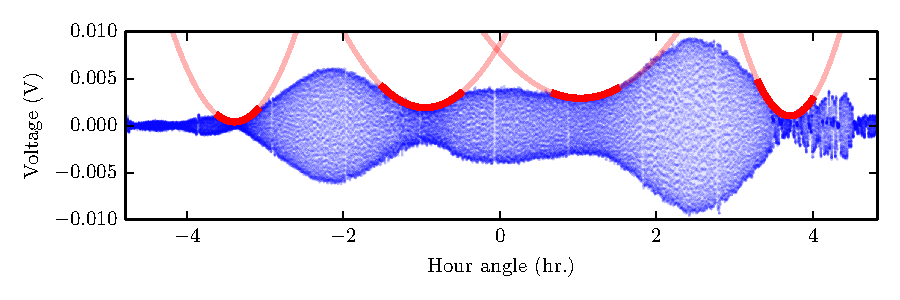
\includegraphics[scale=1]{plots_fitting/sun_minima_all.pdf} \\
    \caption{Fitted envelope minima for sun observation.  Thick red lines plot actual fit within domains, thin red lines extrapolate to illustrate fit shape.}
	\label{fig:sunMinima}
\end{figure}

\begin{figure}[!ht]
    \centering
    \includegraphics[scale=1]{plots_fitting/{sun_modulation_fit_-3.6_-3.1}.pdf} \\
    \includegraphics[scale=1]{plots_fitting/{sun_modulation_fit_-1.5_-0.5}.pdf}
    \caption{Predicted modulation functions from two zero crossings at minima $h_s = -3.39$ (top) and $h_s = -0.95$ (bottom) for sun observation; vertical dotted lines identify minima.  Solid black lines plot our suggested modulation functions, dashed and dotted lines plot modulation functions corresponding to other candidate radii.}
    \label{fig:sunMFfits}
\end{figure}

We assume that modulation function minima correspond to zero crossings of $J_1(z)$, where $z = 2\pi f_f R$.  From various tabulations, $J_1(z)$ has zeros $z_0 = 3.8317$, $z_1 = 7.0156$, $z_2 = 10.1735$, $\ldots$.  Candidate source radii are then $R_i = z_i / (2\pi f_f)$, $i \in \ints^+$.  How do we select or identify the best radius?  Each candidate radius requires a certain shape (and some number of minima) for the modulation function.  For the sun, we expect to see two sets of minima (reflected across zero hour angle) in the correct modulation function; for the moon, we expect only one set.  This is a bit of a charade, so let's be honest.  We're trying to make the shoe fit our misshapen feet (Figure~\ref{fig:sunMFfits}) -- i.e., eyeballing and seeing which shape best fits our data.

We suggest that the outside minima for the sun correspond to the 2nd zero of $J_1$; the inside minima correspond to the 3rd zero of $J_1$ (Figure~\ref{fig:sunMFfits}).  We did not fit minima at lower fringe frequencies (larger hour angle), as the signal was increasingly inconsistent and did not increase in amplitude as expected.  The average of four values of Sun radius (from four minima) is $R_{\mt{sun}} = 0.29\degree$.  We are unable to determine uncertainty, but we note that the candidate radii differ by $\sim0.1\degree$; if our eyeballing procedure is justified, $0.1\degree$ should be a conservative bound on our error.

\begin{figure}[!ht]
    \centering
    \includegraphics[scale=1]{plots_fitting/{moon_modulation_fit_-3.8_-2}.pdf}
    \caption{Predicted modulation functions from minimum $h_s = -3.33$ for 2014 April 4 moon observation.  Vertical dotted lines identifies fitted minimum.  Solid black line plots our suggested modulation function, dashed and dotted lines plot modulation functions corresponding to other candidate radii.}
	\label{fig:moonMFfits}
\end{figure}

The 2014 April 4 moon observation yields a more equivocal choice of modulation functions (Figure~\ref{fig:moonMFfits}).  The black curve appears to describe the data well, but the averaged radius $R_{\mt{moon}} = 0.159\degree$ significantly underestimates the actual moon radius.  The next possible modulation function, corresponding to the second zero of $J_1(z)$, gives $R_{\mt{moon}} = 0.29\degree$.  We disfavor the higher order modulation function due to the apparent lack of minima for hour angle between $[-2, 2]$, despite the closer agreement with the expected modulation function (as the moon and sun should have $R \sim 0.25\degree$).  Data with clearer zero crossings (i.e., less noise) would better determine the appropriate modulation function and hence radius.

% ==========
% Discussion
% ==========
\section{Discussion}

Our modulation function fitting is very sketchy.  Ideally, we should characterize and remove interferometer noise and check interferometer pointing to ensure that we are recording a significant signal, particularly for near-horizon pointing.  Previous iterations of the class have obtained data with slightly different envelope curves, which might better fit our expected modulation functions [\href{http://ugastro.berkeley.edu/radio/interferometer/}
{ugastro.berkeley.edu/radio/interferometer/}].

Our lunar eclipse observation of the Moon was not so useful.  The fringe modulation function should decrease in amplitude during the eclipse due to cooling of the moon's surface [e.g., \textit{Pettit and Nicholson}, 1930]; observing the moon's cooling could allow us to characterize thermal properties of the moon's surface.  However, we first need to be able to accurately model the moon's modulation function outside of an eclipse -- this function will depend on the phase of the moon as well, but will at least have negligible thermal time dependence.  As our other moon observation was taken during a crescent moon ($\sim22\%$ illumination), we suggest follow-up observations during a full moon and a new moon.  The next new moon is 2014 April 28; the next full moon is 2014 May 14.

\begin{figure}[!ht]
    \centering
    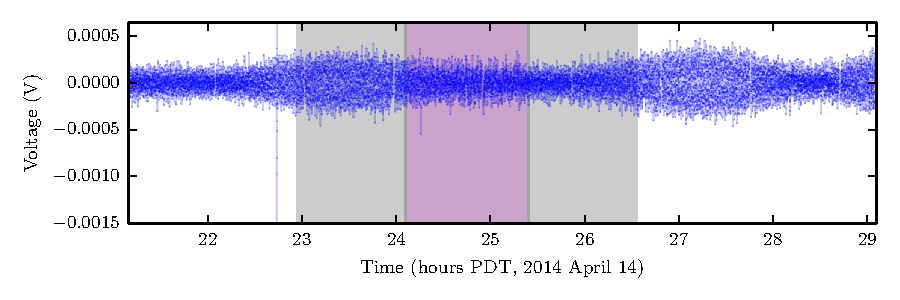
\includegraphics{plots/moon_eclipse_nice_clean.pdf} \\
    \caption{Reduced interferometer data from 2014 April 14 moon observation.  Partial and total eclipse times are highlighted in gray and magenta.}
    \label{fig:eclipse}
\end{figure}

It is worth mentioning that finite frequency bandwidth contributes an extra factor of $\mathrm{sinc} (\Delta\nu\tau)$ to the interferometer's extended source response [\textit{Condon and Ransom}, 2006].  For our interferometer, the argument $\Delta\nu\tau < 1$ and so this term has a relatively small effect.

% ===========
% Conclusions
% ===========
\section{Conclusions}

We successfully fit and estimate various astronomical parameters from interferometer fringe output.  Future work should focus on characterizing interferometer electronics, noise, and pointing to improve data processing and interpretation.  The material presented here naturally leads in to study of more sophisticated arrays and correlators, although our presentation is fairly elementary.

\section{Acknowledgments}

Karto and Baylee's work on the interferometer hardware and software (especially the IDL-Python porting) made this entire lab possible.

\section{Electronic supplement}

All supporting files are stored on the repository:\\
\href{https://github.com/aarontran/ay121}
{https://github.com/aarontran/ay121/lab3/}.

In particular, our repository provides figures generated for all observations but not herein reproduced.

I also note that the lab suggests that we perform a numerical function to determine the best angular radius.  Here I have turned to tabulated Bessel function zeros.  I did perform the numerical integration; candidate radii estimates from two procedures agree to within $0.001\degree$.  The code for this procedure might be found in some old commit though I make no guarantees.  It is straightforward enough, anyways.

\section{References}

\hangindent 0.25in Condon, J. J. and S. M. Ransom (2006), Essential Radio Astronomy, \\
\href{http://www.cv.nrao.edu/course/astr534/ERA.shtml}
{http://www.cv.nrao.edu/course/astr534/ERA.shtml}.

\hangindent 0.25in Dutt, A. and V. Rokhlin (1993), Fast Fourier transforms for
nonequispaced data, \textit{SIAM J. Sci. Comput.}, \textit{14}(6),
1368--1393, doi:10.1137/0914081.

\hangindent 0.25in Ferraz-Mello, S. (1981), Estimation of periods from
unequally spaced observations, \textit{Astrophys. J.}, \textit{86}(4),
619--624, doi:10.1086/112924.

\hangindent 0.25in Green, R. M. (1985), \textit{Spherical astronomy}, 520pp.,
Cambridge Univ. Press, Cambridge.

\hangindent 0.25in Hafez, Y. A. et al. (2014), A radio determination of the time of the New Moon, \textit{Mon. Not. Roy. Astron. Soc.}, \textit{439}(3), 2271--2280, doi:10.1093/mnras/stt2476.

\hangindent 0.25in Pettit, E. and S. B. Nicholson (1930), Lunar radiation and temperatures, \textit{Astrophys. J.}, \textit{71}, 102--135, doi:10.1086/143236.

\hangindent 0.25in Salomonovich, A. E. and B. Y. Losovskii (1963), Radio-brightness distribution on the lunar disk at 0.8 cm, \textit{Soviet Astron.}, \textit{6}(6), 833--839.

\end{document}